\chapter{Diseño del sistema propuesto}
\label{chapter:disenio}

\chapquote{Si tienes tanto miedo al fracaso, nunca tendrás éxito. Tienes que arriesgarte.}{Mario Andretti}

\section{Descripción del caso de estudio} \label{section:CasoEstudio}


\section{Diseño del sistema}


\section{Buffer}

Diagrama ER

\begin{sidewaysfigure}[h]
    \centering
    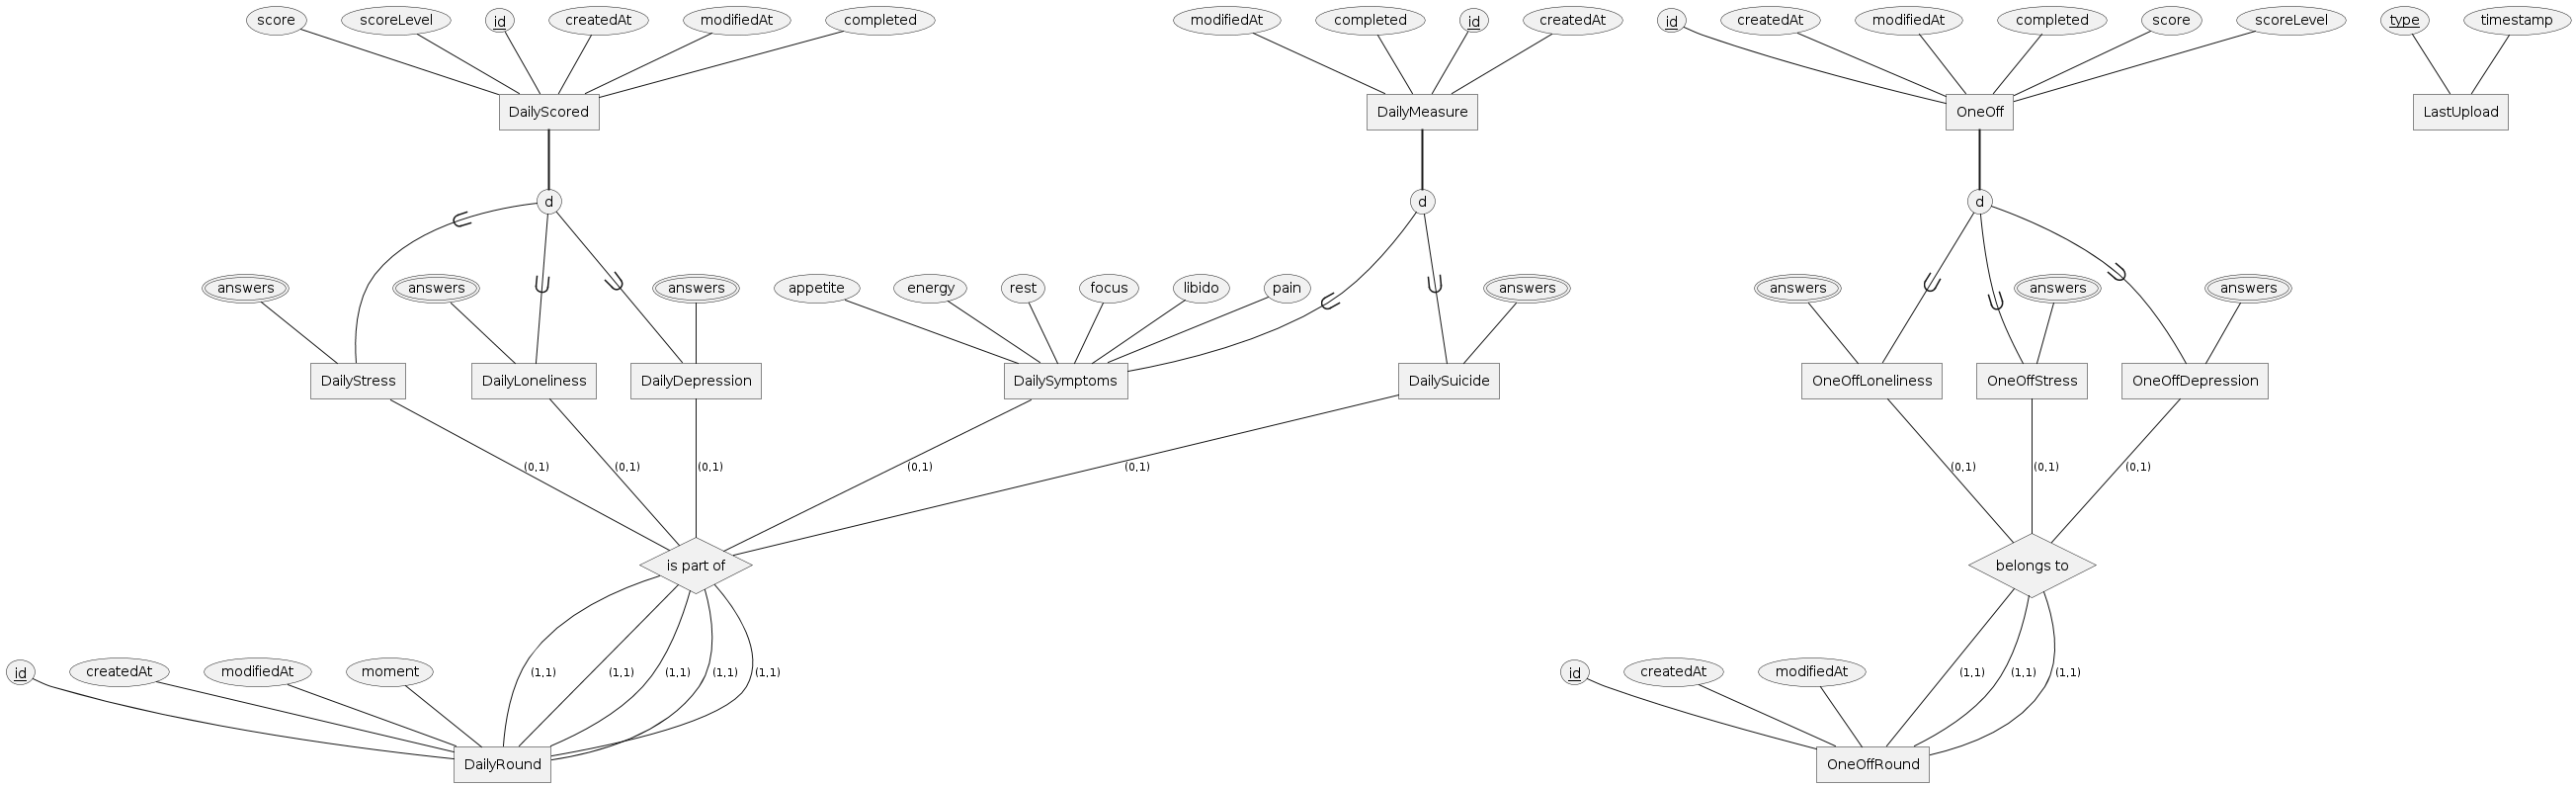
\includegraphics[width=1\textwidth]{figures/bd/ER simple.png}
    \caption[Diagrama ER]{Diagrama ER. Elaboración propia}
    \label{figure:disenio:diagrama_er}
\end{sidewaysfigure}

Diagrama colección datos usuario (\textit{user data})

\begin{figure}[h]
    \centering
    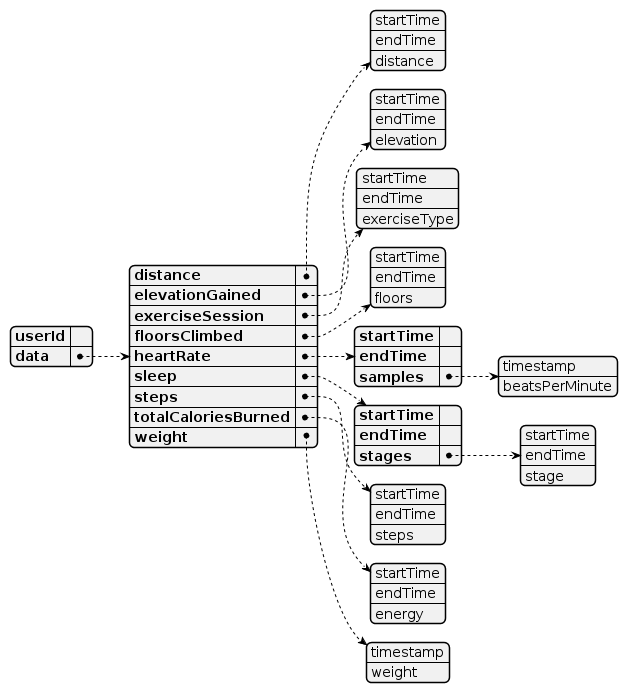
\includegraphics[width=0.75\textwidth]{figures/bd/Servidor user data.png}
    \caption[Diagrama colección datos usuario]{Diagrama colección datos usuario. Elaboración propia}
    \label{figure:disenio:diagrama_user_data}
\end{figure}

Diagrama colección cuestionarios diarios (\textit{daily questionnaires})

\begin{figure}[h]
    \centering
    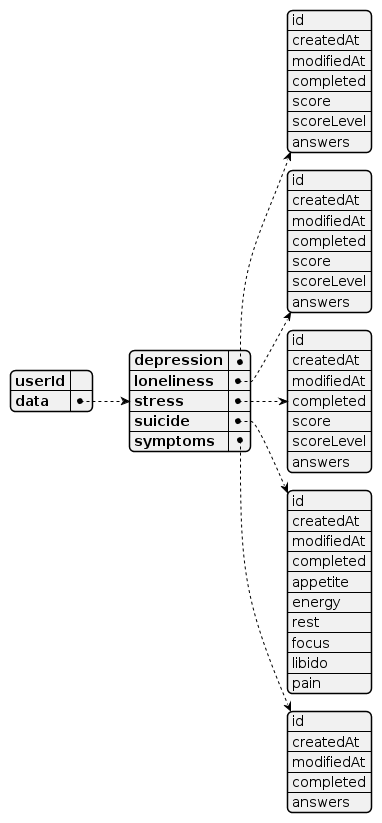
\includegraphics[width=0.33\textwidth]{figures/bd/Servidor daily questionnaires.png}
    \caption[Diagrama colección cuestionarios diarios]{Diagrama colección cuestionarios diarios. Elaboración propia}
    \label{figure:disenio:diagrama_daily}
\end{figure}

Diagrama colección cuestionarios puntuales(\textit{one off questionnaires})

\begin{figure}[h]
    \centering
    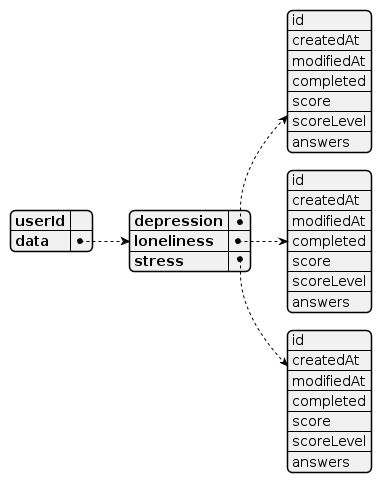
\includegraphics[width=0.33\textwidth]{figures/bd/Servidor one off questionnaires.png}
    \caption[Diagrama colección cuestionarios puntuales]{Diagrama colección cuestionarios puntuales. Elaboración propia}
    \label{figure:disenio:diagrama_one_off}
\end{figure}